\documentclass[]{scrartcl}
\title{Vorlesung Analysis II}
\usepackage{amsmath,amssymb,amsfonts}
\usepackage{stmaryrd}
\usepackage{mathtools}
\usepackage{latexsym}
\usepackage{graphicx}
\usepackage{tikz}
\usepackage{xcolor}
\usepackage[most]{tcolorbox}
\usepackage{soul}
\usepackage{ upgreek }
\usepackage{hyperref}
\usepackage{tipa}
\usepackage[dvipsnames]{xcolor}
\hypersetup{
	colorlinks=true,
	linkcolor=blue,
	filecolor=magenta,      
	urlcolor=cyan,
	pdftitle={Overleaf Example},
	pdfpagemode=FullScreen,
}
\newcommand{\redcircle}[1]{%
	\tikz[baseline=(char.base)]{
		\node[shape=circle, draw=red, text=red, thick, inner sep=1pt] (char) 
		{\textbf{#1}};
	}%
}
\newcommand{\bluecircle}[1]{%
	\tikz[baseline=(char.base)]{
		\node[shape=circle, draw=blue, text=blue, thick, inner sep=1pt] (char) 
		{\textbf{#1}};
	}%
}
\newcommand{\blackcircle}[1]{%
	\tikz[baseline=(char.base)]{
		\node[shape=circle, draw=black, text=black, thick, inner sep=1pt] 
		(char) 
		{\textbf{#1}};
	}%
}
\newcommand{\orangecircle}[1]{%
	\tikz[baseline=(char.base)]{
		\node[shape=circle, draw=orange, text=orange, thick, inner sep=1pt] 
		(char) 
		{\textbf{#1}};
	}%
}
\newcommand{\redul}[1]{\setulcolor{red}{\ul{#1}}}
\newcommand{\blueul}[1]{\setulcolor{blue}{\ul{#1}}}
\newcommand{\yelul}[1]{\setulcolor{yellow}{\ul{#1}}}
\newcommand{\greenul}[1]{\setulcolor{green}{\ul{#1}}}
\newcommand{\oraul}[1]{\setulcolor{orange}{\ul{#1}}}
\setul{1pt}{3pt} % Linienhöhe und Abstand zum Text (optional anpassbar)

\setlength{\topmargin}{-.5in} \setlength{\textheight}{9.25in}
\setlength{\oddsidemargin}{0in} \setlength{\textwidth}{6.8in}
\setlength{\parindent}{0pt}

\begin{document}
	\maketitle
	
	\textbf{\underline{Teil 2: Topologische Grundbegriffe un metrischen Räumen}}\\
	\\
	\textbf{\underline{an10: Konvergenz in metrischen Räumen}}\\
	\\
	\textbf{\underline{\underline{Stichworte:} Normierter $\mathbb{R}-VR$, B-W, Äquivalenz aller Normen im $\mathbb{R}^n$, metrischer Raum,  Kgz im metrischen Raum}}\\
	\\
	\textbf{\underline{Literatur:}} \blueul{[Forster], Kapitel 1,2}\\
	\\
	\textbf{10.1. \underline{Einleitung:}} Wir haben den $\mathbb{R}^n$ mit der Maximumsnorm $||\cdot||_\infty$ versehen und damit die Grenzwerttheorie des $\mathbb{R}^n$ aufgebaut. Die euklidische Norm $||\cdot||_2$ ist dazu äquivalent. Wir beschreiben noch andere Normen, zeigen den mehrdimensionalen Satz von Bolzano-Weierstrß und damit, dass alle Normen im $\mathbb{R}^n$ äquivalent sind.\\
	\\
	\textbf{10.2. \underline{Def.:}} Sei $p\in\mathbb{R}, p\geq 1$. Für $x=(\xi_1,...,\xi_n)^T\in\mathbb{R}^n$ sei $||x||_p:=(\sum_{j=1}^{n}|\xi_j||^p)^{\frac{1}{p}}$ die \redul{p-Norm} bzw. \redul{$l_p-$Norm} bzw. \redul{Hölder-Norm.}\\
	\\
	\textbf{10.3. \underline{Bem.:}} Für p=2 stimmt diese mit der in \blueul{an 1.6} definierten euklidischen Norm überein.\\
	\\
	\textbf{10.4. \underline{Satz:}} \greenul{$||\cdot||_p$ ist eine Norm.}\\
	\underline{Bew.:} Zeigen Eigenschaften \blueul{(N1)-(N3)} in \blueul{an 1.5}, und \blueul{(N1),(N2)} sind klar.\\
	Zu \blueul{(N3)}: Seien $x,y\in\mathbb{R}^n$. Ist $p=1$, dann ist $||x+y||_1=||x||_1+||y||_1$ klar.\\
	Ist $p\textgreater1$, def. q durch $\frac{1}{p}+\frac{1}{q}=1$, d.h. $q=\frac{p}{p-1}=1+\frac{1}{p-1}\textgreater1$.\\
	dann ist $||x+y||_p^p=\sum_{j=1}^{n}|\xi_j+\eta_j|\cdot|\xi_j+\eta_j|^{p-1}\leq\sum_{j=1}^{n}|\xi_j|\cdot|\xi_j+\eta_j|^{p-1}+\sum_{j=1}^{n}|\eta_j|\cdot|\xi_j+\eta_j|^{p-1}\\
	\stackrel{\blackcircle{*}}{\leq}||x||_p(\sum_{j=1}^{n}|\xi_j+\eta_j|^{q(p-1)})^{1/q}+||y||_p(\sum_{j=1}^{n}|\xi_j+\eta_j|^{q(p-1)})^{p-1}\\
	=(||x||_p+||y||_p)\cdot(||x+y||_p)^{p/q}$, also \redul{$||x+y||_p\leq||x||_p+||y||_p.$}\\
	\strut\hfill$\square$\\
	In \blackcircle{*}: Für $a,b \in \mathbb{R}^n$ ist \oraul{$\sum_{j=1}^{n}|\alpha_j\beta_j\leq||a||_p\cdot||b||_q$}, denn \textopencorner$\OE||a||_p=||b||_q=1$\textcorner es gilt:\\
	$\forall \alpha, \beta \leq \frac{\alpha^p}{p}+\frac{\beta^q}{q}$. \textopencorner$\alpha\beta=l^{ln(\alpha)}l^{ln(\beta)}=\exp(\frac{1}{p}ln(\alpha^p)+\frac{1}{q}ln(\alpha^q))\leq \frac{1}{p}l^{ln(\alpha^p)}+\frac{1}{q}l^{ln(\beta^q)}\checkmark$\textcorner\\
	\\
	\textbf{10.5. \underline{Bem.:}} Man nennt die $\triangle$- Unglg. \blueul{(N3)} für $||\cdot||_p$ auch \redul{Minkowski-Ungleichung}.\\
	Die folgende Beh. zeigt, warum man die Maximumsnorm $||x||_\infty:=\max_{1\leq j \leq n}|\xi_j|$ mit dden $\infty$-Zeichen im Index schreibt:\\
	\\
	\textbf{10.6. \underline{Beh.:}} $\forall x\in \mathbb{R}^n: $\greenul{$\lim\limits_{p\rightarrow\infty}||x||_p=||x||_\infty$}.\\
	\underline{Bew.:} Wähle $j\in\{1,...,n\}$ mit $||x||_\infty=|\xi_j|=:M$. sei $\OE x\neq 0.$\\
	Dann gilt $M=(|\xi_j|^p)^{\frac{1}{p}}\leq ||x||_p$ = \oraul{$(\sum_{j=1}^{n}|\xi_j|^p)^{1/p}\leq (nU^p)^{1/p}$} =$n^{1/p}M \xrightarrow{p\rightarrow\infty}1\cdot M.$\\
	\strut\hfill$\square$\\
	\textbf{10.7. \underline{Def.:}} Eine Folge $(x_k)\subseteq \mathbb{R}^n$ heißt \redul{beschränkt} $:\Leftrightarrow (||x_k||_\infty)_{k\in\mathbb{N}}$ beschränkt (in $\mathbb{R}$)\\
	$\Leftrightarrow \exists M \in \mathbb{R} \forall k \in \mathbb{N}: ||x_k||_\infty \leq M$.\\
	\\
	\textbf{10.8. \redul{Satz von Bolzano-Weierstraß}(im $\mathbb{R}^n$)}:\\
	Jede \greenul{beschränkte Folge} besitzt ein \greenul{Konvergente Teilfolge.}\\
	\underline{Bew.:} Sei ($x_k$) beschränkt.\\
	Es genügt, \underline{z.z.:} $\exists$ Teilfolge $(x_{l(k)})_{k\in\mathbb{N}} \forall j \in \{1,...,n\}: pr_j(k_{l(k)})$ konvergiert.\\
	Dazu sei j fest. Dann ist $(pr_j(x_k))_{k\in \mathbb{N}}$ beschränkt.\\
	Dazu $\exists$ Teilfolge $(x_{l(k)})$ mit $pr_j(x_k)$ Kgt. laut \blueul{1-dim. B-W}.\\
	Wenden dies für j=1,...,n an, erhalte somit Folgen\\
	$\mathbb{N}\supseteq (l_1(k))\supseteq(l_2(k))\supseteq...\supseteq(l_n(k))$, setze $l(k):=l_n(k)$ für alle $k\in\mathbb{N}$.\\
	Die Folge $(x_{l(k)})$ ist eine Konvergente Teilfolge, da sie laut Konstruktion in jeder Komponente Konvergiert (d.h. bzgl. $||\cdot||_\infty$), vgl. \blueul{an 1.12.}\\
	\strut\hfill$\square$\\
	\textbf{10.9. \underline{Bem.:}} p Norm auf $\mathbb{R}^n \Rightarrow \forall x,y \in \mathbb{R}^n:$ \greenul{$|p(x-p(y|\leq p(x-y)))$},\\
	und damit ist \greenul{jede Norm auf $\mathbb{R}^n$ stetig}.\\
	\underline{Bew.:} $\bullet$ Haben $p(x)=p(x-y+y)\leq p(x-y)+p(y) \Rightarrow p(x)-p(y)\leq p(x-y),\\$
	und $ p(y)=p(y-x+x)\leq p(x-y)+p(x)\Rightarrow p(y)-p(x)\leq p(x-y),$\\
	zusammen fplgt $|p(x)-p(y)|=\max(p(x)-p(y), p(y)-p(x))\leq p(x-y).$\\
	$\bullet$ Die Stetigkeit folgt direkt: $\forall x \forall \epsilon \textgreater 0 \exists \delta \textgreater0 \forall y: p(x-y)\textless \delta \Rightarrow p(x)-p(y)\leq \epsilon,$\\
	nämlich nimm $\delta=\epsilon$, dazu ist p(x)-p(y)$\leq p(x-y)\textless \delta = \epsilon$.\\
	\strut\hfill$\square$\\
	\textbf{10.10. \underline{Satz:}} \greenul{Alle Normen auf $\mathbb{R}^n$ sind äquivalent}, d.h. \\
	Sind p,qq beliebige Normen, dann \greenul{$\exists \alpha\beta\in \mathbb{R}: p \leq \alpha q$ und $q\leq \beta p$}.\\
	\underline{Bew.:} Haben Ä-Relation der Normen (refl./symm./transitiv klar).\\
	Daher \oraul{gen. z.z.} Jede Norm ist \oraul{zu $||\cdot||_\infty$ äquivalent}.\\
	\oraul{1. Schritt:} Mit der Standardbasis $e_1,...,e_n$ des $\mathbb{R}^n$ gilt:\\
	$p(x)=p(\sum_j\xi_je_j)\leq \sum_jp(\xi_je_j)= \sum_j|\xi_j|p(e_j)\leq ||x||_\infty \underbrace{\sum_{j=1}^{n}p(e_j)}_{=:a}$\\
	\oraul{2. SChritt:} \underline{Ann.:} $\exists z\in S :\{x\in \mathbb{R}^n; ||x||_\infty= 1\}$ mit $p(z)=\inf_{x\in S}p(x)$.\\
	$\Rightarrow p(z)=min_{x\in S}p(x).$\\
	Dann setze $\frac{1}{\beta} :=p(z)$ (da ja $z\neq 0$).\\
	\underline{Beh.:} Dieses $\beta$ tut's, d.h. $||\cdot||_\infty\leq \beta p.$\\
	Denn: Sei $\OE x\neq 0, y:=\frac{x}{||x||_\infty}\in  S$,\\
	Dann ist $\frac{1}{||x||_\infty} p(x)=p(\frac{1}{||x||_\infty}\cdot x)=p(y)\geq p(z)=\frac{1}{\beta}$\\
	$\Rightarrow ||x||_\infty \leq \beta p(x)$ wie gewünscht.\\
	Zeige also \underline{Annahme:}\\
	Wähle $(x_k)\subseteq S$ mit $p(x_k)\xrightarrow{k\rightarrow \infty}\inf_{e\in S}p(x),$\\
	wegen $(x_k)\subseteq S$ ist $(x_k)$ beschränkt.\\
	Mit \blueul{B-W 10.8} folgt $\lim\limits_{n\rightarrow \infty}x_{l(k)}=z.$\\
	Dann ist $|||x_{l(k)}||_\infty-||z||_\infty|\leq ||x_{l(k)}-z||_\infty \xrightarrow{k\rightarrow \infty}0\Rightarrow||z||_\infty=1.$\\
	Haben somit ein $z\in S$ mit $p(z)=\inf_{x\in S}p(x)$, da p stetig nach \blueul{10.9}.\\
	\newpage
	\textbf{10.11. \underline{Bsp.:}} Einheits"Kugeln" bzgl. verschiedener Normen: Sei $a\in \mathbb{R}^2, \epsilon \textgreater 0$.\\
	\begin{figure}[h]
		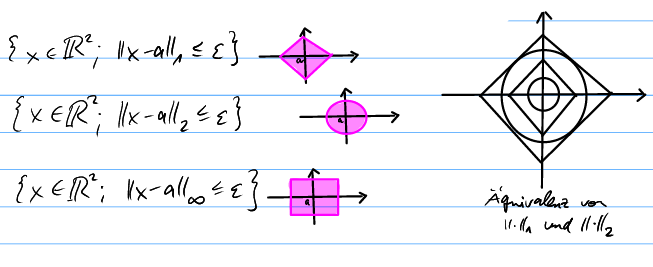
\includegraphics[width=8 cm,height=5cm]{bsp kap 10.11}
	\end{figure}\\
	Zur Abstandsmessung im \redul{Normierten $\mathbb{R}-V$ Räumen} dient der Term $||x-y||\in\mathbb{R}_{\geq 0}$.\\
	\\
	\textbf{10.12. \underline{Def.:}} In einem endlich dim. normierten $\mathbb{R}-VR$ ($\mathbb{R}^n,||\cdot||$) heißt die Abb. \yelul{$\delta$} :$\mathbb{R}^nx\mathbb{R}\rightarrow \mathbb{R}_{\geq0},$ \yelul{$\delta(x,y)$} :=\redul{$||x-y||$} die \redul{zu $||\cdot||$ gehörige Metrik.}\\
	\\
	\textbf{10.13. \underline{Bem.:}} Die zu $||\cdot||$ gehörige Metrik erfüllt die folgende Eigenschaften:\\
	(M1)\greenul{$\delta(x,y)=0 \Leftrightarrow x=y$}, denn $\delta(x,y)=0\Leftrightarrow||x-y||=0\Leftrightarrow x-y=0 \Leftrightarrow x=y.$\\
	(M2)\greenul{$\delta(x,y)=\delta(y,x)$}, denn $\delta(x,y)=||x-y||=||-(y-x)||=|-1|\cdot||y-x||=||y-x||=\delta(y,x)$.\\
	(M3) \greenul{$\delta(x,z)\leq\delta(x,y)+\delta(y,z)$}, denn $\delta (x,z)=||x-z||=||(x-y)+(y-z)||\leq||x-y||+||y-z||=\delta(x,y)+\delta(y,z).$\\
	\\
	Diese drei Grundeigenschaften der "Abstandsmessung" sind ohne Angabe einer Norm formulierbar, wir sprechen dann allgemein von einem \redul{metrischen Raum.}\\
	\\
	\textbf{10.14. \underline{Def.:}} Sei R eine Menge und $\delta: R \times R\rightarrow\mathbb{R}_{\geq 0}$ eine Abb. mit den Eigenschaften\\
	(M1)$\forall x,y \in R: \delta (x,y)=0 \Leftrightarrow x=y$\\
	(M2) $\forall x,y \in R: \delta(x,y=\delta y,x)$ \redul{(Symmetrie)}\\
	(M3) $\forall x,y,z \in R: \delta(x,z)\leq\delta(x,y)+\delta(y,z)$ \redul{$\triangle$-Unglg.}\\
	Dann heißt $\delta$ eine \redul{Metrik} (auf R) und $(R,\delta)$ ein \redul{metrischer Raum}.\\
	\\
	\textbf{10.15. \underline{Folgerung:}}(1) \greenul{$|\delta(a,b)-\delta(x,y)|\leq \delta(a,x)+\delta(b,y) $}\\
	(2) \greenul{$|\delta(a,b)-\delta(a,y)|\leq \delta(b,y)$}.\\
	\underline{Bew.:} (1): $\delta(a,b) \leq \delta(a,x)+\delta(x,b)\leq\delta(a,x)+\delta(x,y)+\delta(y,b)$\\
	$\Rightarrow ßdelta(a,b) -\delta(x,y)\leq \delta (a,x)+\delta(b,y)$,\\
	analog: $\delta(x,y)-\delta(a,b)\leq\delta(a,x)+\delta(b,y).\\$
	(2): Setze x=a in \blueul{(1)}.\\
	\strut\hfill$\square$\\
	Konvergenz dann in metrischen Räumen erklärt werden. Sei dazu \yelul{$(R,\delta)$} \underline{metrischer Raum.}\\
	\\
	\textbf{10.16. \underline{Def.:}} Eine Folge $(x_k)\subseteq R$ \redul{konvergiert} gegen $a\in R :\Leftrightarrow \lim\limits_{k\rightarrow\infty} \delta(x_k,a)=0.$\\
	\underline{Notation:} $x_k \xrightarrow{k\rightarrow \infty}a$ bzw. $\lim\limits_{k\rightarrow\infty}x_k=a.$\\
	Nennen a den \redul{Grenzwert} der Folge ($x_k$) in R, kurz: GW.\\
	\\
	\textbf{10.17. \underline{Eigenschaften} der Konvergenz im metrischen Raum:}\\
	(1) $x_k\rightarrow a, x_k\rightarrow b \Rightarrow a=b$ (\redul{Eindimensional des GW})\\
	(2) $x_k \rightarrow a, y_k\rightarrow b\Rightarrow \lim\limits_{k\rightarrow \infty \delta(x_k,y_k)=\delta(a,b)}$ \redul{(Stetigkeit der Metrik)}.\\
	\underline{Bew.:} Zu (1): $a=b\leftrightarrow \delta(a,b)=0,$ aber: $\delta(a,b)\leq \delta(a,x_k)+\delta(x_k,b)\xrightarrow{k\rightarrow\infty}0+0=0$.\\
	\underline{Zu (2):} $|\delta(x_k,y_k)-\delta(a,b)|\leq \delta(a,x_k)+\delta(b,y_k)\xrightarrow{k\rightarrow \infty}0+0=0.$\\
	\\
	\textbf{10.18. \underline{Def.:}} Eine Folge $(x_k)\subseteq R$ in einem metrischen Raum $(r,\delta)$ heißt \redul{Cauchyfolge}:$\Leftrightarrow \forall \epsilon\textgreater 0 \exists k_0\in \mathbb{N} \forall k,l \in \mathbb{N}, k,l\geq k_0: \delta(x_k,x_l)\textless\epsilon.$\\
	\\
	\textbf{10.19. \underline{Satz:}} Jede \greenul{Konvergente Folge $(x_k)\subseteq R$ ist eine Cauchyfolge.}\\
	\underline{Bew.:} Klar, geht genauso wie in \blueul{An 5.21.}\\
	\\
	\textbf{10.20. \underline{Def.:}} Ein metrischer Raum R heißt \redul{vollständig}, wenn jede Cauchyfolge Konvergiert. \textopencorner vgl. \blueul{An 6.9}\textcorner\\
	\\
	wir zeigen nun, dass jeder normierter endlich-dimensionale $\mathbb{R}-VR$ vollständig ist.\\
	(bemerke, dass jeder n-dimensionale $\mathbb{R}-VR$ zu $\mathbb{R}^n$ isomorph ist, \blueul{s. Lin. Algebra}).\\
	\\
	\textbf{10.21. \underline{Satz:}} Es sei $||\cdot||:\mathbb{R}^n\rightarrow\mathbb{R}_{\geq0}$ \greenul{irgendeine Norm} auf $\mathbb{R}^n$, \greenul{$\delta(x,y)=||x-y$}.\\
	Dann ist \greenul{($\mathbb{R}^n,\delta$) ein vollständiger Raum.}\\
	\underline{Bew.:} Bekannt aus \blueul{10.10}: $\exists M_1,M_2\textgreater0 \forall x \in\mathbb{R}^n: ||x||\leq M_1||x||_\infty, ||x||_\infty\leq M_2||x||$\\
	Sei $(x_k)$ eine Cauchyfolge bzgl. $\delta$. Sei $\epsilon\textgreater0$, dann $\exists k_0\in\mathbb{N}:\delta(x_k,x_l)\textless \frac{\epsilon}{M_2},$\\
	d.h. $||x_k-x_l||\textless \epsilon$ wegen $\frac{||x_k-x_l||_\infty}{M_2}\leq||x_k-x_l||=\delta(x_k,x_l)$ für alle $k,l\geq k_0$.\\
	Daraus folgt: $|pr_j(x_k)-pr_j(x_l)|\textless \epsilon$ für alle $j\in\{1,...,n\}$,\\
	d.h. $(pr_j(x_k))_{k\in\mathbb{N}}$ ist eine Cauchyfolge in $\mathbb{R}$.\\
	da$\mathbb{R}$ vollständig ist (vgl. \blueul{An. 6.9}), gilt: $\exists\alpha_j\in\mathbb{R}:\lim\limits_{k\rightarrow\infty}pr_j(x_k)=\alpha_j$.\\
	Setze $a:=(\alpha,...,\alpha_n)^T\in\mathbb{R}^n$. Dann gilt $\lim\limits_{k\rightarrow\infty}x_k=a$,\\
	denn $\delta(x_k,a)=||x_k-a||\leq M_1||x_k-a||_\infty = M_1\max_{1\leq j \leq n}|pr_j(x_k)-\alpha_j|\xrightarrow{k\rightarrow\infty}0.$\\
	\strut\hfill$\square$\\
	\textbf{10.22. \underline{Bsp.:}} $\bullet (\mathbb{R}^2,||\cdot||_2)$ ist vollständiger $\mathbb{R}-VR$ der Dimension 2. $\bullet$($\mathbb{Q},|\cdot|$) ist nicht vollständig.\\
	$\bullet (l[a,b],||\cdot||_{sup})$ ist vollständig, $(l[a,b], ||\cdot||_1)$ ist nicht vollständig, vgl. \redcircle{Ü} Nl.1 A4, Bl. 2 A5.
	
		
\end{document}